\documentclass{article}
\usepackage{amsmath}
\usepackage{mathtext}
\usepackage[english,russian]{babel}
\usepackage[T2A]{fontenc}
\usepackage[utf8]{inputenc}
\usepackage{graphicx}
\graphicspath{{img/}}
\DeclareGraphicsExtensions{.jpg, .png, .pdf}
\begin{document}
\section{Сложные передачи планетарные передачи}

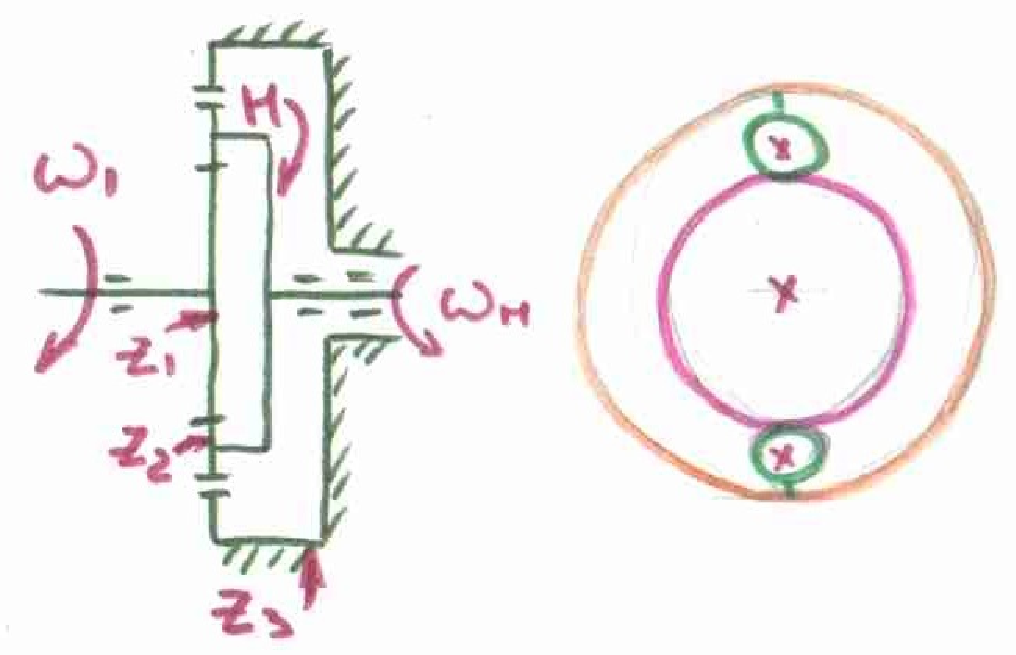
\includegraphics[width = \textwidth]{1}

\underline{Планетарными} называются передачи, состоящие из зубчаных колес и вращающихся звеньев, на которых располагаются оси зубчатых колес.

Звено на котором располагаются подвижные оси колес, нвызвается водило H, А зубчатые колеса с подвижными осями наз. сателитами. Колесо с неподвижной осью вращения $z_1$ называется солнечным. Неподвижное колесо $z_3$ наз. опорным (или короткой).

Расчет передаточного отношения планетарной передачи методами обращенного движения (Формула Смирнова-Виллиса).

\begin{tabular}{ccc}
	& Исходное & Обращенное\\
	солнечное колесо $z_1$ & $\omega_1$ & $\omega_1 - \omega_н$\\
	сателит $z_2$ & $\omega_2$ & $\omega_2 - \omega_н$\\
	водило H & $\omega_н$ & 0\\
	опорное колесо $z_3$ & $\omega_1$ & $- \omega_н$\\
\end{tabular}
$$
i_{1\:н} = \frac{\omega_1}{\omega_н}
$$
$$
i_{13}^{(н)} = \frac{\omega_1 - \omega_н}{- \omega_н}  = 1 - \frac{\omega_1}{\omega_н} = 1 - i_{1н}
$$
$$
i_{13}^{(н)} = \frac{z_3}{z_2} \left(- \frac{z_2}{z_1} \right) = - \frac{z_3}{z_1}
$$
\underline{Выбор числа зубьев}:
\begin{enumerate}
	\item Число зубьев дожно обеспечивать передаточное отношение $i_{1н}$
	\item Должно обеспечиваться условие соосности: $d_3 - d_1 = 2 d_2$, $z_3 - z_1 = 2 z_2$
	\item Должно обеспечиваться условие сборки: $\frac{z_1 + z_3}{K} = целое число$, k - число сателитов.
	\item Должно обеспечиваться условие соседства
\end{enumerate}
\underline{Достоинства}:
\begin{enumerate}
	\item Соостность входного и выходного вала
	\item Легкость получения большого передаточного отношения без существенного увеличения габаритов.
	\item В зацеплении могут находиться одновременно несколько пар зубьев зубчатых колес, что удменьшает нагрузку на пару зубчатых колес и уменьшает маодуль, а, следовательно, и уменьшает габариты.
	\item Наличие нескольких пар зацепления зубьев обеспечивает снижение погрешности кинематической и обеспечивает плавность хода
\end{enumerate}
\underline{Недостатки}:
\begin{enumerate}
	\item Резкий спад КПД при очень большом передаточном отношении.
\end{enumerate}
\end{document}
